\chapter{Instantiating cognitive models for automotive applications}
\begin{itemize}
	\item example tasks
	\item data sets
	\item labelling/training data generation
	\item implementation in \ac{Nengo}
	\item implementation details
\end{itemize}
\section{Driving context classification}
\label{sec:driving_context_class}
Fig. \ref{subfig:system_arch} shows a schematic overview of our system architecture. 
\textit{Environment perception} happens through a variety of different sensors \cite{Aeberhard2015} providing \textit{preprocessed data} in the form of object-lists or raw sensory data.
We build our representation from this preprocessed data through \textit{vectorization} of sensory data and high-level object lists.
We use a \textit{neural network} for predictions based on the current scene vector.
Here, we use supervised learning to distinguish three different driving contexts, namely city, interurban and highway.
\subsection{Training data}
The input data used for training and evaluating the system is real-world data gathered during test drives in the region of Munich, Germany. 
Depending on the test vehicle's sensor setup \cite{Aeberhard2015}, a subset of the following sensor systems is available: camera, RADAR, LIDAR as well as the dynamics of the ego-vehicle (e.g. velocity, acceleration, steering angle) through introspective sensors. 
While lists of dynamic objects (i.e. cars, pedestrians, etc.) are available from all extrospective sensors, the camera-based perception system additionally provides lists of static objects like traffic signs. 
In this work, we focus on the ego-vehicle's dynamics and the information provided by the camera-system as the only extrospective sensor. 
The camera-system is present in all available test traces and furthermore, its data is most informative regarding categories of dynamic objects while being the only system that provides information about traffic signs. 
Beside the object's classification, the camera systems provides estimations (with variance) of entities like relative position, orientation and velocity for each object. 
The data is divided into three different sets: one for training and two test sets containing roughly \SIlist{27;18;7}{\minute} respectively of driving data.\\
To enable automated training of any supervised learning system, the training data needs to be labeled. 
In this section, we hand-labeled our data sets by visually inspecting the images provided by a reference camera-system and labelling the intervals  between transitions of driving contexts as indicated by the respective traffic signs. 
\subsection{Scene representation in vectors}
\begin{figure}[t!]
	\centering
	\subfloat[Example scene with labeled object vectors based on environment perception\label{subfig:ex_scene}]{%
		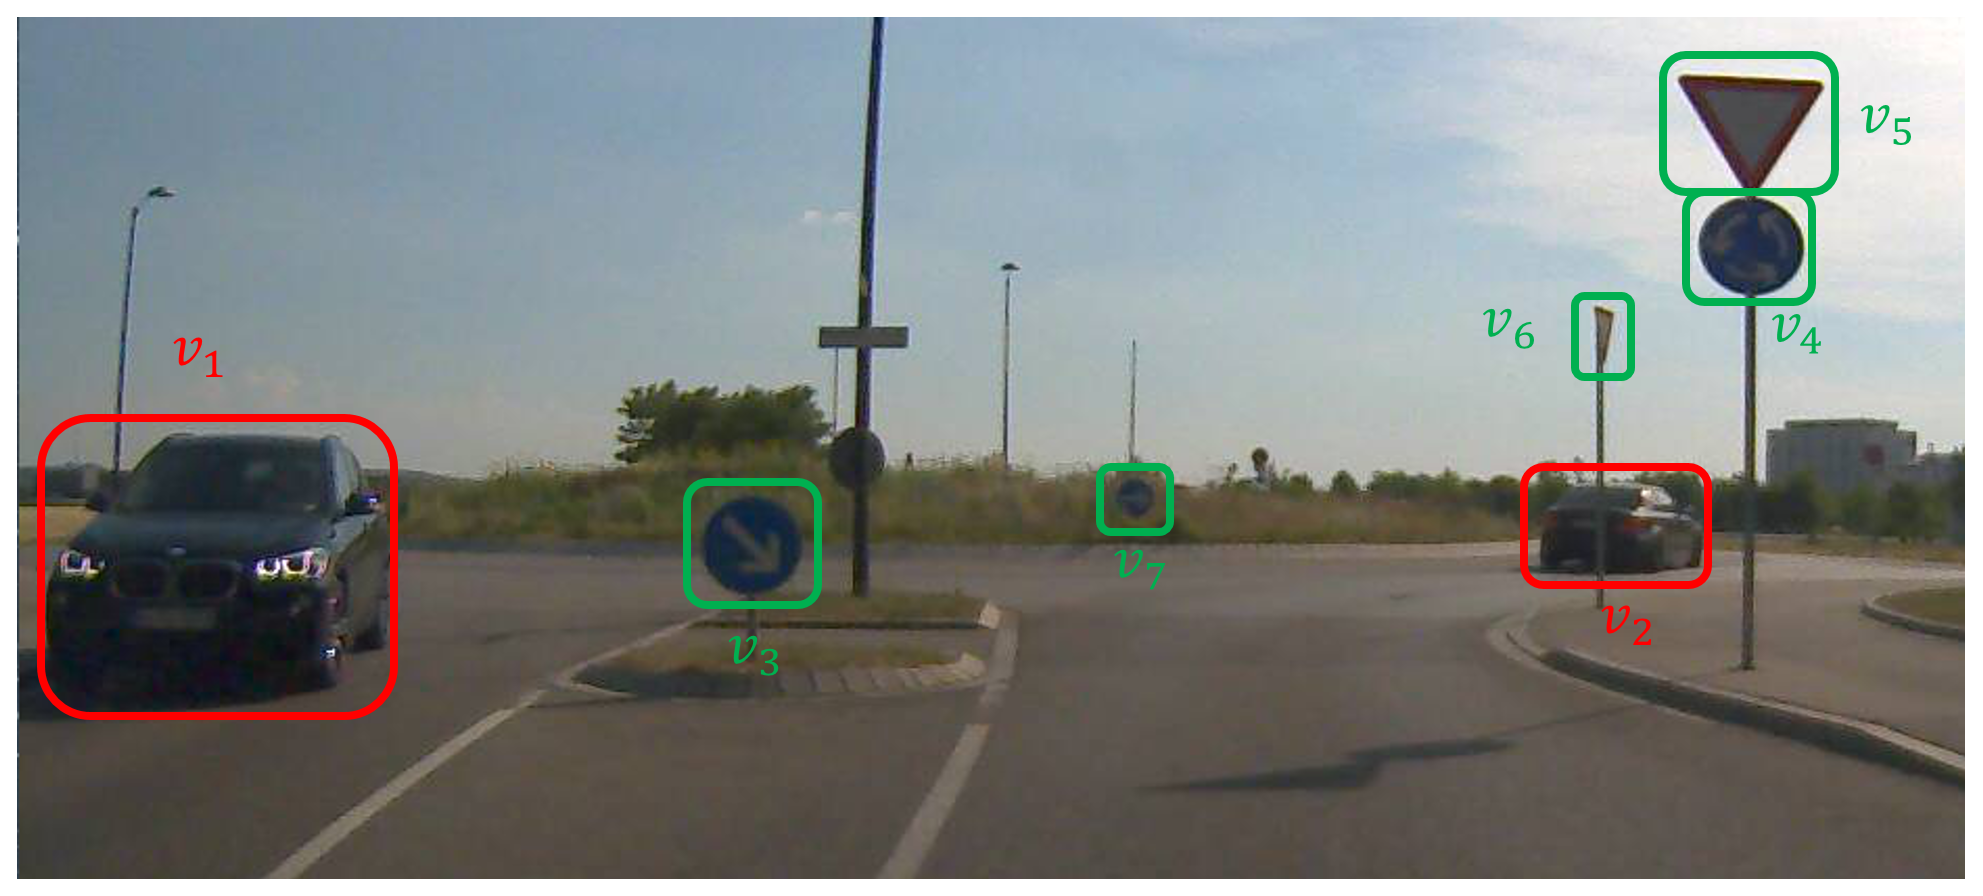
\includegraphics[width=0.45\textwidth, height=3.2cm]{imgs/Example_scene.eps}
	}
	\subfloat[System architecture\label{subfig:system_arch}]{%
		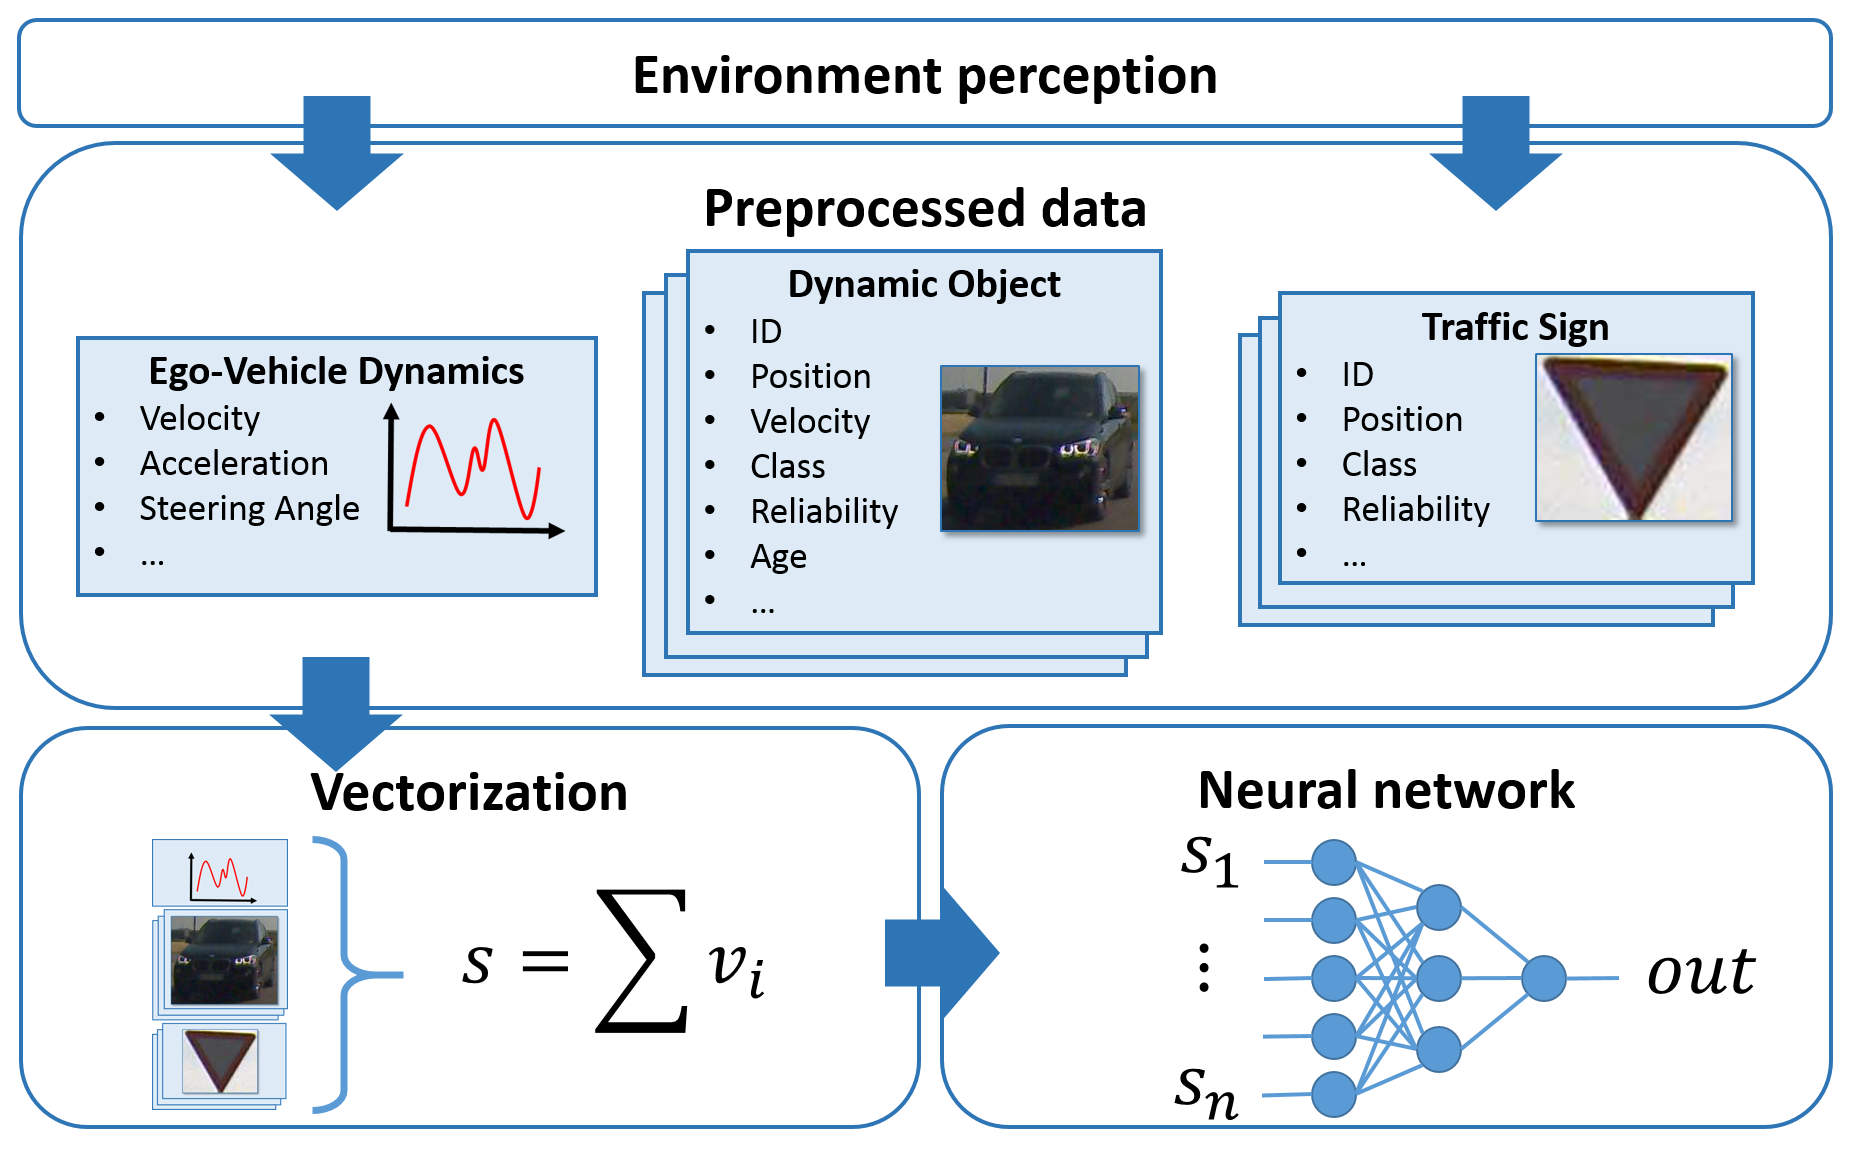
\includegraphics[width=0.45\textwidth, height=3.2cm]{imgs/system_overview_horizontal.eps}
	}
	\caption{Schematic system overview with one example scene.}\label{fig:sys}
\end{figure}
For this application, we encapsulate three types of information in our vector-based scene representation: ego-vehicle dynamics , dynamic objects and traffic signs (provided as preprocessed object-lists).
For each category, we describe the process of converting the input data into a vector representation. 
We obtain the final vector describing the current scene by superposition of all vectors created in each category. 
For all our vectors in this work we have chosen a dimension of $D=512$, a reasonable trade-off between informational capacity and computational complexity.\\
%\subsubsection{Ego-vehicle dynamics}
%\label{subsubsec:ego-veh-dyn}
\subsubsection{Ego-vehicle dynamics} 
For ego-vehicle dynamics, we use the current velocity, acceleration in $x$/$y$-direction (ego-vehicle coordinate system), the angle of the steering wheel as well as the steering angle of the front axle. 
For all values except acceleration, we randomly choose one normalized ID-vector representing the respective value, e.g. $\mathbf{VELOCITY}=\left(v_1, \cdots, v_D\right)$ with $v_i \in \mathbb{R}$ for velocity, and multiply this ID-vector with the current scalar value $x$, e.g. $x \cdot \mathbf{VELOCITY}$ for velocity.
Furthermore, we normalize all scalar values to the range $\left[-2,2\right]$ to keep the length of our vectors limited.
For vectorization of two-dimensional values, we use an encoding with sine and cosine functions with different spatial frequencies and offsets. 
Therefore, we define the following helper functions
\[ \abb{f_{\left(m,i\right)}}{\mathbb{R}^2}{\mathbb{R}^4}{\left(x,y\right)}{\left(\cos\frac{m\cdot \pi + x}{i + 1}, \sin\frac{m\cdot \pi + x}{i + 1}, \cos\frac{m\cdot \pi + y}{i + 1}, \sin\frac{m\cdot \pi + y}{i + 1}\right)},
\]
\[
\abb{\psi_i}{\mathbb{R}^2}{\mathbb{R}^4}{\left(x,y\right)}{\left(f_{\left(0,i\right)}\left(x,y\right), f_{\left(\frac{1}{2},i\right)}\left(x,y\right), f_{\left(1,i\right)}\left(x,y\right), f_{\left(\frac{3}{2},i\right)}\left(x,y\right)\right)}
\]
and obtain the final vector representation of acceleration in $x$/$y$-direction via the function
\[
\abb{\lambda}{\mathbb{R}^2}{\mathbb{R}^D}{\left(x,y\right)}{\frac{1}{\sqrt{\frac{D}{2}}}\left(\psi_0\left(x,y\right), \cdots, \psi_{\frac{D}{16}-1}\left(x,y\right)\right).}
\]
This encoding $\lambda\left(a_x, a_y\right)$ leads to normalized, nonzero, similar vectors with information distributed over all elements (in contrast to a simple encoding like $\left(a_x, a_y, 0 \cdots, 0\right)$).\\
%\subsubsection{Dynamic Objects}
\subsubsection{Dynamic objects} 
The camera-based classification system is able to distinguish seven different object categories, namely bicycle, car, motorcycle, pedestrian, stationary, truck and unknown.
In the simplest form of our vector representation, we assign one random vector to each of those categories and add it to the current scene representation once for each category's occurrence in the object-list. 
However, this representation just encodes that there are certain objects present somewhere in the current scene without any additional information.
Enhancing this simple encoding, we use the function $\lambda$ to map each dynamic object's position in $x$/$y$-direction (relative to the ego-vehicle) to vector form and bind the result to the vector representing the object's category. 
%However, position information might not be that informative regarding the task of distinguishing between driving contexts. 
One quite unique feature of e.g. highway driving is the fact that almost all other traffic participants drive in similar direction as the ego-vehicle.
Therefore, we create additional random vectors encoding the orientation of dynamic objects relative to the ego-vehicle for three discretized categories, namely $\mathbf{SAME}$, $\mathbf{OPPOSITE}$ and $\mathbf{LATERAL}$. 
%We can now bind this orientation information to each dynamic object as we did for position information. 
If we want to jointly bind those two pieces of information to one object, we need to introduce two additional ID-vectors $\mathbf{POSITION}$ and $\mathbf{ORIENTATION }$ to impose structure. 
For example, a car detected at position $\left(p_x,p_y\right)$ with approximately the same orientation as the ego-vehicle would lead to the following vector representation
\[ 
\mathbf{CAR} + \mathbf{CAR}\otimes\mathbf{POSITION}\otimes\lambda\left(p_x,p_y\right) + \mathbf{CAR}\otimes\mathbf{ORIENTATION}\otimes\mathbf{SAME}.
\]
%\subsubsection{Traffic Signs}
\subsubsection{Traffic signs} 
The ego-vehicle's camera-system \cite{Aeberhard2015} is able to recognize a significant amount and variety of traffic signs. 
Again, we assign a random vector to each possible traffic sign label and add it to the current scene representation. 
However, in contrast to dynamic objects, most traffic signs are not only valid while being visible but stay relevant for the current driving context until withdrawn by another sign. 
Therefore, we implemented a simple form of memory for a certain subset of traffic signs relevant to the task of driving context classification even after disappearing. %, namely speed limit signs as well as signs indicating "environmental changes" like e.g. entrance/exit of a city or highway. 
Due to the fact, that the camera system is not immune to false detections, we implemented a decaying memory, to avoid relying too much on false detections and to allow the system to consider other cues. 
We realized the decay by multiplying each vector representing a traffic sign with a (parameterizable) scalar decay factor  at each time step. 
Furthermore, we included a simple withdraw logic, e.g. new speed limit signs overwrites previously seen ones and a sign indicating a city entrance withdraws a memorized highway sign.\\
%\subsection{Training}
\subsection{Baseline for classification: human level performance}
To get a better understanding of the quality of the context classification system's results, we compare it to human level performance.
However, neither showing raw camera images nor numerical vectors would yield comparable results.
Therefore, we created human-readable versions of our input vectors in text form and presented a subset of $50$ random samples for each data set (with the training set always being the first) to two human subjects asking for their classification guess.
\subsection{Experimental results}
\section{Behaviour prediction}
Predicting future behaviour and positions of other traffic participants from observations is a key problem, that needs to be solved by human drivers and automated vehicles alike to safely navigate their environment and to reach their desired goal.
Therefore, we picked behaviour prediction as another task for investigating the potential of vector representations in automotive context.
In contrast to the previous task of classifying the current driving context (cf. Sec. \ref{sec:driving_context_class}), predicting future positions of vehicles is a regression problem, as we are predicting continuous values (spatial positions) instead of discrete labels.
However, future positions of vehicles not only depend on each vehicle's own past positions and dynamic data (e.g. velocity and acceleration) but also on the behaviour of the other traffic participants in the vehicle's surroundings.
There exist various different approaches to account for those interactions between traffic participants or, more generally, agents in the scene: probabilistic models like costmaps \cite{Bahram2016} accounting for physical constraints on the movements, categorizing and representing scenes in a hierarchy \cite{Bonnin2012}, modeling the interactions in the learning network architecture \cite{Alahi2016} or including distances between other agents and the target directly in the training data \cite{Altche2018}.
We hypothesize that structured vector representations will be able to capture these relations and mutual influence between traffic participants, which is necessary for reliable predictions.
As we aim for a model-free data representation, we neglect 
In a second example task, we use our vector representation as input data for a neural network to predict the future position of one other traffic participant at a time.
We use an indication vector $\mathbf{THIS}$ bound to the object we want to predict to tell the network the current focus.
To predict all objects of the scene during deployment, we envision to use multiple instantiations of the same network.
Thereby, the amount of training data generated per file increases with the number of objects while we only need to train one network.
\subsection{Training data}
The data used for the behaviour prediction task is real-world data gathered during test drives in the region of Munich, Germany.
In total, there are \SI{27}{\hour} of driving time available in our data set.
The largest part of this data is collected while driving on German highways.
\todo{check if newer files from leo are available with traffic sign or traffic rules in them}
\begin{itemize}
	\item describe data set
	\item find interesting slice in the data set
	\item labelling/training data generation
\end{itemize}
\subsubsection{Performance baselines}
In this section, we analyze
\begin{figure}[t!]
	\centering
	\subfloat[Overtaking maneuvre at $t=\SI{90}{\second}$\label{subfig:overtaking1}]{%
		\includegraphics[clip,width=\columnwidth]{imgs/Vis_overtaking_maneuvre_t1.png}
	}
	
	\subfloat[Overtaking maneuvre at $t=\SI{94}{\second}$\label{subfig:overtaking2}]{%
		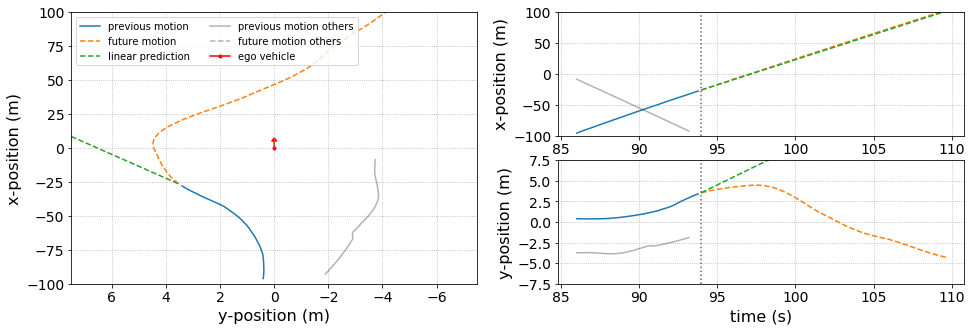
\includegraphics[width=\columnwidth]{imgs/Vis_overtaking_maneuvre_t2.png}
	}
	\caption{An example of an overtaking maneuvre in a highway situation. The ego-vehicle is overtaken by another car approaching from behind. Subfigures \ref{subfig:overtaking1}--\ref{subfig:overtaking4} show different times of the maneuvre. Solid lines indicate previous positions whereas dashed lines indicate future positions or predictions. The dashed green line illustrates linear predicions based on a constant velocity assumption for $x$ direction and linear regression using the last \SI{0.5}{\second} of the positions for $y$ direction.} \label{fig:overtaking1}
\end{figure}	
\begin{figure}[t!]
	\subfloat[Overtaking maneuvre at $t=\SI{98}{\second}$\label{subfig:overtaking3}]{%
			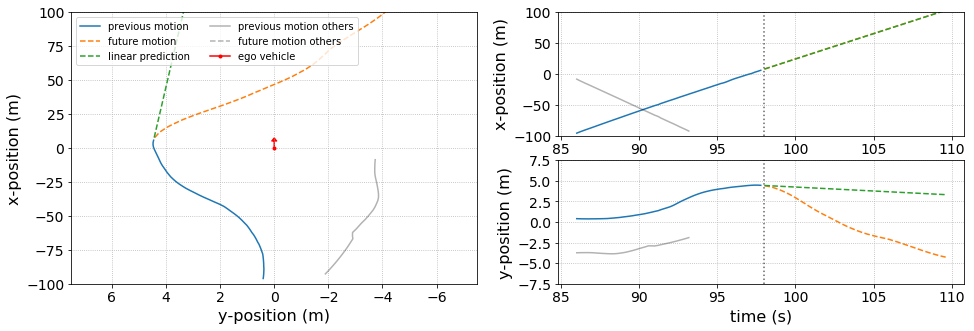
\includegraphics[width=\columnwidth]{imgs/Vis_overtaking_maneuvre_t3.png}
	}
	
	\subfloat[Overtaking maneuvre at $t=\SI{100}{\second}$\label{subfig:overtaking4}]{%
			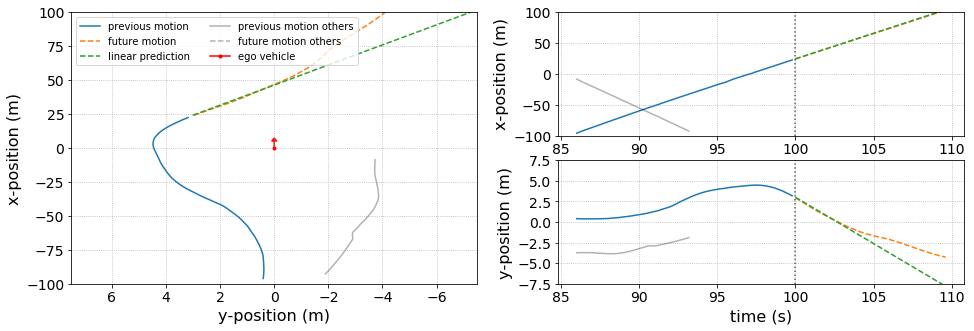
\includegraphics[width=\columnwidth]{imgs/Vis_overtaking_maneuvre_t4.png}
	}	
	\caption{An example of an overtaking maneuvre in a highway situation. The ego-vehicle is overtaken by another car approaching from behind. Subfigures \ref{subfig:overtaking1}--\ref{subfig:overtaking4} show different times of the maneuvre. Solid lines indicate previous positions whereas dashed lines indicate future positions or predictions. The dashed green line illustrates linear predicions based on a constant velocity assumption for $x$ direction and linear regression using the last \SI{0.5}{\second} of the positions for $y$ direction.}\label{fig:overtaking2}
\end{figure}
\begin{itemize}
	\item linear regression
	\item kalman filters?
	\item something else?
\end{itemize}
\subsubsection{Labelling}

\subsection{Scene representation in vectors}
\subsection{Offline (batch) learning}
\subsection{Refinement at runtime through online learning}
\subsection{Experimental results}
\section{Other applications}